\documentclass[12pt, a4paper]{amsart}

\usepackage{picture}
\usepackage{amsthm}
\usepackage{amssymb}
\usepackage{amsmath, exercise}
\usepackage[activeacute, spanish]{babel}
\usepackage[utf8]{inputenc}
\usepackage{mathpazo}
\usepackage[pdftex]{color, graphicx}
\usepackage{fancyhdr}
\usepackage{multicol}
\usepackage{tikz-cd}
\usepackage{mathrsfs}
\usepackage{pstricks}
\usepackage[colorlinks=true]{hyperref}
\usetikzlibrary{calc}
\usetikzlibrary{matrix}

\usepackage{enumitem}

\usepackage[margin=0.8in]{geometry}

\usepackage{pgfplots}
\pgfplotsset{compat=1.13}
\usepackage{tikz}
\usetikzlibrary{arrows}
\usetikzlibrary{patterns}

\usepackage{booktabs}
\usepackage{float}
\usepackage{multirow}
\usepackage{subfig}

\newtheorem{teo}{Teorema}[]
\newtheorem{lem}[teo]{Lema}
\newtheorem{prop}[teo]{Proposición}
\newtheorem{cor}[teo]{Corolario}

\newtheorem*{propnonumber}{Proposición}

\theoremstyle{definition}
\newtheorem{prob}[teo]{Problema}
\newtheorem{conj}[teo]{Conjectura}
\newtheorem{defn}[teo]{Definición}
\newtheorem{ax}[teo]{Axioma}
\newtheorem{ex}[teo]{Ejemplo}
\newtheorem{exer}[teo]{Ejercicio}

\newtheorem*{obs}{Observación}
\newtheorem*{com}{Comentario}
\newtheorem*{defnonumber}{Definición}

\newcommand{\bd}[1]{\mathbf{#1}}  % for bolding symbols
\newcommand{\CC}{\mathbb{C}}
\newcommand{\RR}{\mathbb{R}}      % for Real numbers
\newcommand{\ZZ}{\mathbb{Z}}      % for Integers
\newcommand{\NN}{\mathbb{N}}
\newcommand{\QQ}{\mathbb{Q}}
\newcommand{\FF}{\mathbb{F}}
\newcommand{\mm}{\mathfrak{m}}
\newcommand{\col}[1]{\left[\begin{matrix} #1 \end{matrix} \right]}
\newcommand{\comb}[2]{\binom{#1^2 + #2^2}{#1+#2}}
\newcommand{\eps}{\varepsilon}
\newcommand{\norm}[1]{\left\| #1 \right\|}
\newcommand{\abs}[1]{\left\lvert #1 \right\rvert}
\newcommand{\pint}[1]{\left\langle #1 \right\rangle}
\newcommand{\tendsto}[1]{\xrightarrow{\smash{\raisebox{-2ex}{$\scriptstyle#1$}}}}
\newcommand*\diff{\mathop{}\!\mathrm{d}}
\renewcommand{\hom}{\mathrm{Hom}}

\renewcommand{\hom}{\mathrm{Hom}}
\let\oldemptyset\emptyset
\let\emptyset\varnothing
\DeclareMathOperator{\id}{id}
\DeclareMathOperator{\mcm}{mcm}
\DeclareMathOperator{\mcd}{mcd}
\DeclareMathOperator{\ord}{ord}
\DeclareMathOperator{\nil}{nil}
\DeclareMathOperator{\im}{im}
\DeclareMathOperator{\End}{End}
\DeclareMathOperator{\Aut}{Aut}
\DeclareMathOperator{\sg}{sg}
\DeclareMathOperator{\coker}{coker}
\DeclareMathOperator{\Obj}{Obj}
\DeclareMathOperator{\rank}{rk}
\DeclareMathOperator{\gr}{gr}
\DeclareMathOperator{\car}{car}
\DeclareMathOperator{\Nil}{Nil}
\DeclareMathOperator{\Spec}{Spec}
\DeclareMathOperator{\ev}{ev}
\DeclareMathOperator{\ann}{Ann}
\DeclareMathOperator{\Gal}{Gal}
\DeclareMathOperator{\HH}{H}
\DeclareMathOperator{\rg}{rg}
\def\acts{\curvearrowright}
\def\stca{\curvearrowleft}

\def\noteson{%
\gdef\note##1{\marginpar[##1]{##1}}}
\gdef\notesoff{\gdef\note##1{}}
\noteson

\renewcommand{\qed}{\hfill \mbox{\raggedright \rule{0.075in}{0.075in}}}
\renewcommand{\thefootnote}{[\arabic{footnote}]}

\usepackage{scrextend}% not needed with a KOMA-Script class, provides the
                      % `addmargin' environment

\usepackage[load-headings]{exsheets}
\DeclareInstance{exsheets-heading}{mylist}{default}{
  runin = true ,
  attach = {
    main[l,vc]number[l,vc](-2em,0pt) ; % 3em = indent of question body
    main[r,vc]points[l,vc](\linewidth+\marginparsep,0pt)
  }
}

\SetupExSheets{
  headings = mylist , % use the new headings instance
  headings-format = \textbf ,
  counter-format = qu ,
  counter-within = section
}


\usepackage{etoolbox}
% 3em = indent of question body :
\AtBeginEnvironment{question}{\addmargin[2em]{0em}}
\AtEndEnvironment{question}{\endaddmargin}

\usepackage{lipsum}

\begin{document}

\title{Geometría Diferencial -- 1er cuatrimestre 2017}
\author{}
% Remove command to get current date 
\date{}
\nocite{*}
%\begin{abstract}
%\end{abstract}
\maketitle
\begin{center}
\section*{Práctica 1: Variedades y funciones diferenciables}
\end{center}

\textsl{\textbf{Generalidades}}
\vspace{1em}


\begin{question}
Probar que los siguientes conjuntos tienen una estructura de variedad diferencial, exhibir un atlas y hallar la dimensión en cada caso.
\begin{enumerate}[label=\textbf{\alph*.}]
\item Un espacio vectorial $V$ sobre $\RR$.
\item La esfera $S^n\subseteq\RR^{n+1}$.
\item El espacio proyectivo $\mathbb{P}^n(\RR) = S^n / \sim$, donde $x\sim y$ si $x=- y$.
\item El toro $T_n = S^1\times\cdots\times S^1$.
\item El cilindro $\{(x,y,z)\in\RR^3:x^2+y^2=1\}$.
\item El grupo general lineal $\mathrm{GL}_n(\RR)=\{A\in\mathrm{M}_n(\RR):\det(A)\neq 0\}$.
\item El grupo especial lineal $\mathrm{SL}_n(\RR)=\{A\in\mathrm{M}_n(\RR):\det(A)=1\}$.
\item El grupo ortogonal $\mathrm{O}_n(\RR) = \{A\in\mathrm{M}_n(\RR):A\cdot A^\intercal=1\}$.
\item El grupo especial ortogonal $\mathrm{SO}_n(\RR)=\{A\in\mathrm{O}_n(\RR) : \det(A)=1\}$.
\end{enumerate}
\end{question}

\begin{question}
Sea $M$ una variedad diferencial de dimensión $d$ y sea $U\subseteq M$ abierto. 
\begin{enumerate}[label=\textbf{\alph*.}]
\item Probar que $U$ hereda una estructura de variedad con $\dim(U)=\dim(M)$ y que la inclusión $U\hookrightarrow M$ es diferenciable para esa estructura.
\item Probar que un subconjunto $S\subseteq M$ (con la topología subespacio) es una variedad de dimensión $d$ si y sólo si $S$ es abierto en $M$.
\end{enumerate}
\end{question}

\begin{question}
Sea $M$ una variedad diferencial conexa. Probar que para cada par de puntos $p,q\in M$ existe un camino suave $c:[0,1]\to M$ que los une (es decir, $c$ es una función continua en $[0,1]$, diferenciable en $(0,1)$, y $c(0)=p$, $c(1)=q$).
\end{question}

\begin{question}
Sean $M,N$ variedades diferenciales. Probar que una función $f:M\to N$ es diferenciable si y sólo si $g\circ f:N\to\RR$ es diferenciable para toda $g:N\to\RR$ diferenciable.
\end{question}

\begin{question}
Sea $M$ una variedad diferencial y $\pi:S^n\to\mathbb{P}^n(\RR)$ la proyección canónica. Probar que $f:\mathbb{P}^n(\RR)\to M$ es diferenciable si y sólo si $f\circ p:S^n\to M$ es diferenciable. Comparar el rango de $f$ con el de $f\circ p$.
\end{question}

\begin{question}
Sea $M$ una variedad diferencial de dimensión $d$ y $(U,\phi)$ una carta de $M$.
\begin{enumerate}[label=\textbf{\alph*.}]
\item Probar que si $V\subseteq U$ es un abierto, entonces $(V,\left.\phi\right|_V)$ es una carta compatible de $M$.
\item Probar que si $f:\phi(U)\to V\subseteq\RR^d$ es un difeomorfismo, $(U,f\circ\phi)$ es una carta compatible de $M$.
\end{enumerate}
\end{question}

\begin{question}
Sea $M$ una variedad diferencial de dimensión $d$.
\begin{enumerate}[label=\textbf{\alph*.}]
\item Probar que $M$ admite un atlas $\mathscr{A}=\{(U_i,\phi_i):i\in I\}$ tal que para todo $i\in I$ se tiene que $\phi_i(U_i)$ es un abierto acotado de $\RR^d$.
\item Probar que $M$ admite un atlas $\mathscr{B}=\{(V_j,\psi_j):j\in J\}$ tal que para todo $j\in J$ se tiene que $\psi_j(V_i)=\RR^d$.
\end{enumerate}
\end{question}

\begin{question}
Considerar en $\RR$ las cartas $(\RR,\id)$ y $(\RR,\phi)$ donde $\phi(t)=t^3$. Probar que las dos cartas no son compatibles pero que las variedades definidas por el atlas formado por cada una de las cartas son difeomorfas.
\end{question}

\begin{question}
Sea $M$ la imagen de la función $f:(0,2\pi)\to\RR^2$ donde $f(t)=(\sin(t),\sin(2t))$ con la estructura inducida por la carta $(M,f^{-1})$. Probar que la función $F:M\to M$ definida por $F(x,y)=(x,-y)$ no es diferenciable.
\begin{figure}[h]
\begin{center}
\begin{tikzpicture}
    \draw[ultra thick] (-4,0) -- (-4+2*pi,0);
    \draw[ultra thick, red] (-4+1/4*pi,0) -- (-4+1/2*pi,0);
    \draw[ultra thick, yellow] (-4+3/4*pi,0) -- (-4+pi,0);
    \draw[ultra thick, blue] (-4+5/4*pi,0) -- (-4+3/2*pi,0);
    \draw[ultra thick, green] (-4+7/4*pi,0) -- (-4+2*pi,0);
		\node [label=below:$0$,draw,fill=black,circle,inner sep=0pt,minimum size=2pt] at (-4,0) {};
		\node [label=below:$\dfrac{\pi}{4}$,draw,fill=black,circle,inner sep=0pt,minimum size=2pt] at (-4+1/4*pi,0) {};
		\node [label=below:$\dfrac{\pi}{2}$,draw,fill=black,circle,inner sep=0pt,minimum size=2pt] at (-4+1/2*pi,0) {};
		\node [label=below:$2\pi$,draw,fill=black,circle,inner sep=0pt,minimum size=2pt] at (-4+2*pi,0) {};
		\node [label=below:$\dfrac{3\pi}{4}$,draw,fill=black,circle,inner sep=0pt,minimum size=2pt] at (-4+3/4*pi,0) {};
		\node [label=below:$\pi$,draw,fill=black,circle,inner sep=0pt,minimum size=2pt] at (-4+pi,0) {};
		\node [label=below:$\dfrac{5\pi}{4}$,draw,fill=black,circle,inner sep=0pt,minimum size=2pt] at (-4+5/4*pi,0) {};
		\node [label=below:$\dfrac{3\pi}{2}$,draw,fill=black,circle,inner sep=0pt,minimum size=2pt] at (-4+6/4*pi,0) {};		
		\node [label=below:$\dfrac{7\pi}{4}$,draw,fill=black,circle,inner sep=0pt,minimum size=2pt] at (-4+7/4*pi,0) {};		
		
		\draw [samples = 500, ultra thick,domain=0:2*pi] plot 
        ({2*sin(\x r)+8},{sin(2*\x r)});
	
		\draw [samples = 500, ultra thick, red, domain = 1/4*pi: 1/2*pi] plot
        ({2*sin(\x r)+8},{sin(2*\x r)});
		
		\draw [samples = 500, ultra thick, yellow, domain = 3/4*pi: pi] plot
        ({2*sin(\x r)+8},{sin(2*\x r)});
		
		\draw [samples = 500, ultra thick, blue, domain = 5/4*pi: 3/2*pi] plot
        ({2*sin(\x r)+8},{sin(2*\x r)});
		
		\draw [samples = 500, ultra thick, green, domain = 7/4*pi: 2*pi] plot
        ({2*sin(\x r)+8},{sin(2*\x r)});
					
		\node [label=above:$f\left(\dfrac{\pi}{4}\right)$,draw,fill=black,circle,inner sep=0pt,minimum size=2pt] at (9.41,1) {};
		\node [label=right:$f\left(\dfrac{\pi}{2}\right)$,draw,fill=black,circle,inner sep=0pt,minimum size=2pt] at (10,0) {};
		\node [label=below:$f\left(\dfrac{3\pi}{4}\right)$,draw,fill=black,circle,inner sep=0pt,minimum size=2pt] at (9.41,-1) {};
		\node [label=above:$f\left(\dfrac{5\pi}{4}\right)$,draw,fill=black,circle,inner sep=0pt,minimum size=2pt] at (8-1.41,1) {};
		\node [label=left:$f\left(\dfrac{3\pi}{2}\right)$,draw,fill=black,circle,inner sep=0pt,minimum size=2pt] at (6,0) {};
		\node [label=below:$f\left(\dfrac{7\pi}{4}\right)$,draw,fill=black,circle,inner sep=0pt,minimum size=2pt] at (8-1.41,-1) {};
				
\end{tikzpicture}
\end{center}
\label{fig::lemniscata}
\end{figure}
\end{question}

\begin{question}
Probar que $SO_3(\RR)$ es difeomorfo al espacio proyectivo $\mathbb{P}^3(\RR)$.
\end{question}

\begin{question}
Probar que $\RR$ y $S^1$ son las únicas variedades diferenciales conexas de dimensión $1$ salvo difeomorfismo.
\end{question}

\textsl{\textbf{Construcción de variedades}}
\vspace{1em}


\begin{question}\textbf{Preimagen de valor regular:} Sean $U\subseteq\RR^n$ un abierto y $F:U\to\RR^m$ ($n\geq m$) una función diferenciable tal que $c\in\RR^m$ es un valor regular de $F$ (es decir, para cada punto $x\in U$ con $F(x)=c$ el rango de $\mathrm{D}F(x)$ es $m$). Probar que $M=F^{-1}(c)$ es una variedad de dimensión $n-m$ y la inclusión $M\hookrightarrow U$ es diferenciable.
\end{question}

\begin{question}\textbf{Producto cartesiano:} Sean $M$ y $N$ variedades diferenciales.
\begin{enumerate}[label=\textbf{\alph*.}]
\item Probar que el producto cartesiano $M\times N$ es naturalmente una variedad diferencial con $\dim(M\times N)=\dim(M)+\dim(N)$ y que las proyecciones canónicas $\pi_1:M\times N\to M$ y $\pi_2:M\times N\to N$ son diferenciables. 

\item El producto de variedades diferenciales está caracterizado por la siguiente \textit{propiedad universal}: Si $P$ es una variedad diferencial junto con funciones diferenciables $p_1:P\to M, p_2:P\to N$ entonces existe una única función diferenciable $f:P\to M\times N$ tal que $\pi_1\circ f = p_1$ y $\pi_2\circ f = p_2$.
\end{enumerate}
\end{question}

\begin{question}
\textbf{Pegado de variedades:} Sea $(M_i)_{i\in I}$ una familia numerable de variedades diferenciales, todas de dimensión $n$. Supongamos que para cada par $i\neq j$ están dados: dos abiertos $U_{ij}\subseteq M_i$ y $U_{ji}\subseteq M_j$, y un difeomorfismo $f_{ij}:U_{ij}\to U_{ji}$ que no puede extenderse continuamente a ningún punto de $\partial U_{ij}$, tales que se satisfacen las siguientes propiedades:
\begin{itemize}
\item $f_{ji}=f_{ij}^{-1}$.
\item $f_{ij}(U_{ij}\cap U_{ik}) = U_{ji}\cap U_{jk}$.
\item $f_{ik} = f_{jk}\circ f_{ij}$ en $U_{ij}\cap U_{ik}$.
\end{itemize}

Mostrar que existe una variedad diferencial $M$ y morfismos $\psi_i:M_i\to M$ tales que $\psi_i$ es un difeomorfismo entre $M_i$ y un abierto de $M$ y
\begin{enumerate}[label=\textbf{\alph*.}]
\item los abiertos $\psi_i(M_i)$ cubren $M$,
\item $\psi_i(U_{ij})=\psi_i(M_i)\cap\psi_j(M_j)$,
\item $\psi_i=\psi_j\circ f_{ij}$ en $U_{ij}$.
\end{enumerate}
\end{question}

\begin{question}
\textbf{Suma conexa de variedades:} Sean $M$ y $N$ dos variedades conexas de la misma dimensión $d$. Se consideran cartas $(U,\phi)$ y $(V,\psi)$ de $M$ y $N$ respectivamente tales que $\phi(U)=\psi(V)=B(0,1)$ y pongamos $p=\phi^{-1}(0)$ y $q=\psi^{-1}(0)$. Definimos una nueva variedad $M\# N$ como el pegado de $M\smallsetminus\{p\}$ y $N\smallsetminus\{q\}$ por los abiertos $U$ y $V$ a través del difeomorfismo $f:U\to V$ determinado por la ecuación $$\psi f\phi^{-1}(x)=\dfrac{1-\norm{x}}{\norm{x}} x \;\;\forall x\in B(0,1)\smallsetminus\{0\}.$$ La variedad $M\# N$ se llama la suma conexa de $M$ y $N$. Convencerse de que esta construcción no depende de las cartas utilizadas.

\noindent Probar que $M\# S^d$ es difeomorfa a $M$ y que la operación $\#$ es conmutativa y asociativa.
\vspace{1em}

\noindent \textit{Observación:} Se puede probar que cualquier variedad compacta de dimensi\'on $2$ es difeomorfa a la esfera $S^2$, a la suma de $n$ toros $T\#\cdots\# T$ o a la suma de $n$ planos proyectivos $\mathbb{P}(\RR)^2\#\cdots\#\mathbb{P}(\RR)^2$. Es m\'as, estas variedades no son homeomorfas entre s\'{\i}.

\begin{figure}[H]
	\centering
		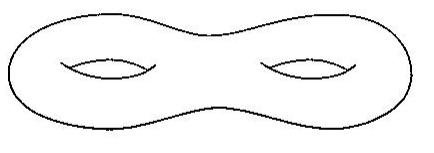
\includegraphics[scale=0.5]{Practica1toro2.jpg}
	\label{fig:Practica1toro2}
\end{figure}

\begin{figure}[H]
	\centering
		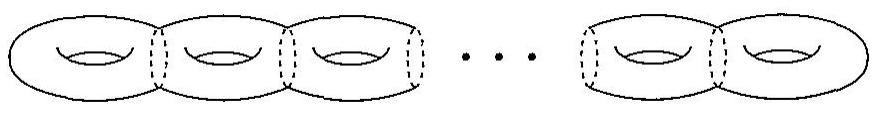
\includegraphics[scale=0.5]{Practica1torog.jpg}
	\label{fig:Practica1torog}
\end{figure}


\end{question}

\begin{question}
\textbf{Cociente por la acción de un grupo:} Sea $M$ una variedad diferencial y $G$ un grupo que actúa en $M$ por difeomorfismos: para cada $g\in G$ se tiene $\phi_g:M\to M$ difeomorfismo de modo que $\phi_{1_G}=1_M$ y $\phi_g\phi_h=\phi_{gh}$. Supongamos además que la acción es propiamente discontinua (es decir, todo $p\in M$ está contenido en un abierto $U$ tal que $\phi_g(U)\cap U=\emptyset$ para todo $g\neq 1_G$) y para todos $p,q\in M$ en distintas órbitas existen abiertos $U$ y $V$ que los contienen respectivamente tales que $\phi_g(U)\cap V = \emptyset$ para todo $g\in G$.
\begin{enumerate}[label=\textbf{\alph*.}]
\item Probar que el conjunto de órbitas $M/G$ es una variedad diferencial con la estructura inducida por $M$, la proyección canónica $M\to M/G$ es diferenciable y $\dim(M)=\dim(M/G)$.
\item Expresar el espacio proyectivo $\mathbb{P}^n(\RR)$ y el toro $n$-dimensional $T_n$ como cocientes $S^n/G$ y $\RR^n/H$ para grupos y acciones convenientes.
\end{enumerate}
\end{question}

\textsl{\textbf{Álgebras de funciones}}
\vspace{1em}


\begin{question}
Probar que $\mathscr{C}^\infty(M,\RR)=\{f:M\to\RR:f\text{ es diferenciable}\}$ es un anillo con la suma y el producto punto a punto. Probar que si $g:M\to N$ es diferenciable, entonces $g^*:\mathscr{C}^\infty(N,\RR)\to\mathscr{C}^\infty(M,\RR)$ es un morfismo de anillos.
\end{question}

\begin{question}
Dadas $M$ y $N$ variedades diferenciales compactas, probar que:
\begin{enumerate}[label=\textbf{\alph*.}]
\item Los ideales maximales de $\mathscr{C}^\infty(M,\RR)$ son de la forma $$\mathfrak{m}_p = \{f\in\mathscr{C}^\infty(M,\RR): f(p)=0\}.$$
\item Todo morfismo de $\RR$-álgebras $\mathscr{C}^\infty(N,\RR)\to\mathscr{C}^\infty(M,\RR)$ viene de una función diferenciable $M\to N$.
\end{enumerate}
\vspace{1em}


\noindent \textit{Observación:} Por \textbf{a.} podemos recuperar la variedad $M$ como conjunto a partir de $\mathscr{C}^\infty(M,\RR)$, por $\textbf{b.}$ también recuperamos su estructura diferenciable. ¿Qué pasa si $M$ y $N$ no son compactas? ¿Vale \textbf{b.} si sólo pedimos morfismo de anillos?
\end{question}

\begin{question}
Probar que el conjunto $\mathscr{D}_p(M)$ de gérmenes de funciones diferenciables a valores reales alrededor de un punto $p\in M$ es un anillo y si $g:M\to N$ es diferenciable entonces $g^*:\mathscr{D}_{g(p)}(N)\to\mathscr{D}_p(M)$ es un morfismo de anillos.
\end{question}

\begin{question}
Dado $p\in M$ probar que la aplicación cociente $f\mapsto\overline{f}$ da un isomorfismo de $\RR$-álgebras $$\mathscr{C}^\infty(M,\RR)/\mathfrak{m}_p^0\to\mathscr{D}_p(M)$$ donde $\mathfrak{m}_p^0 = \{f\in\mathscr{C}^\infty(M,\RR): f \text{ se anula en un entorno de } p\}$.
\vspace{1em}

\noindent\textit{Observación}: Las $\RR$-álgebras $\mathscr{D}_p(M)$ son anillos locales cuyo único ideal maximal son los gérmenes de funciones que se anulan en $p$. Más aún, $\mathscr{D}_p(M)$ es la localización de $\mathscr{C}^\infty(M,\RR)$ en el complemento del ideal maximal $\mathfrak{m}_p$.
\end{question}


\end{document}